% \section{L1 Support in zkSharding: Contracts and Data Availability}
\subsection{L1 Support in zkSharding}
\label{sec:l1}

\todoisinline{We're going directly to typical L2-L1 communication here. I
	think, second section shoud be more related to uniqueness of our
	project

	\handan{Now, it as a subsection of the Overview section}}

\begin{figure}
	\centering
	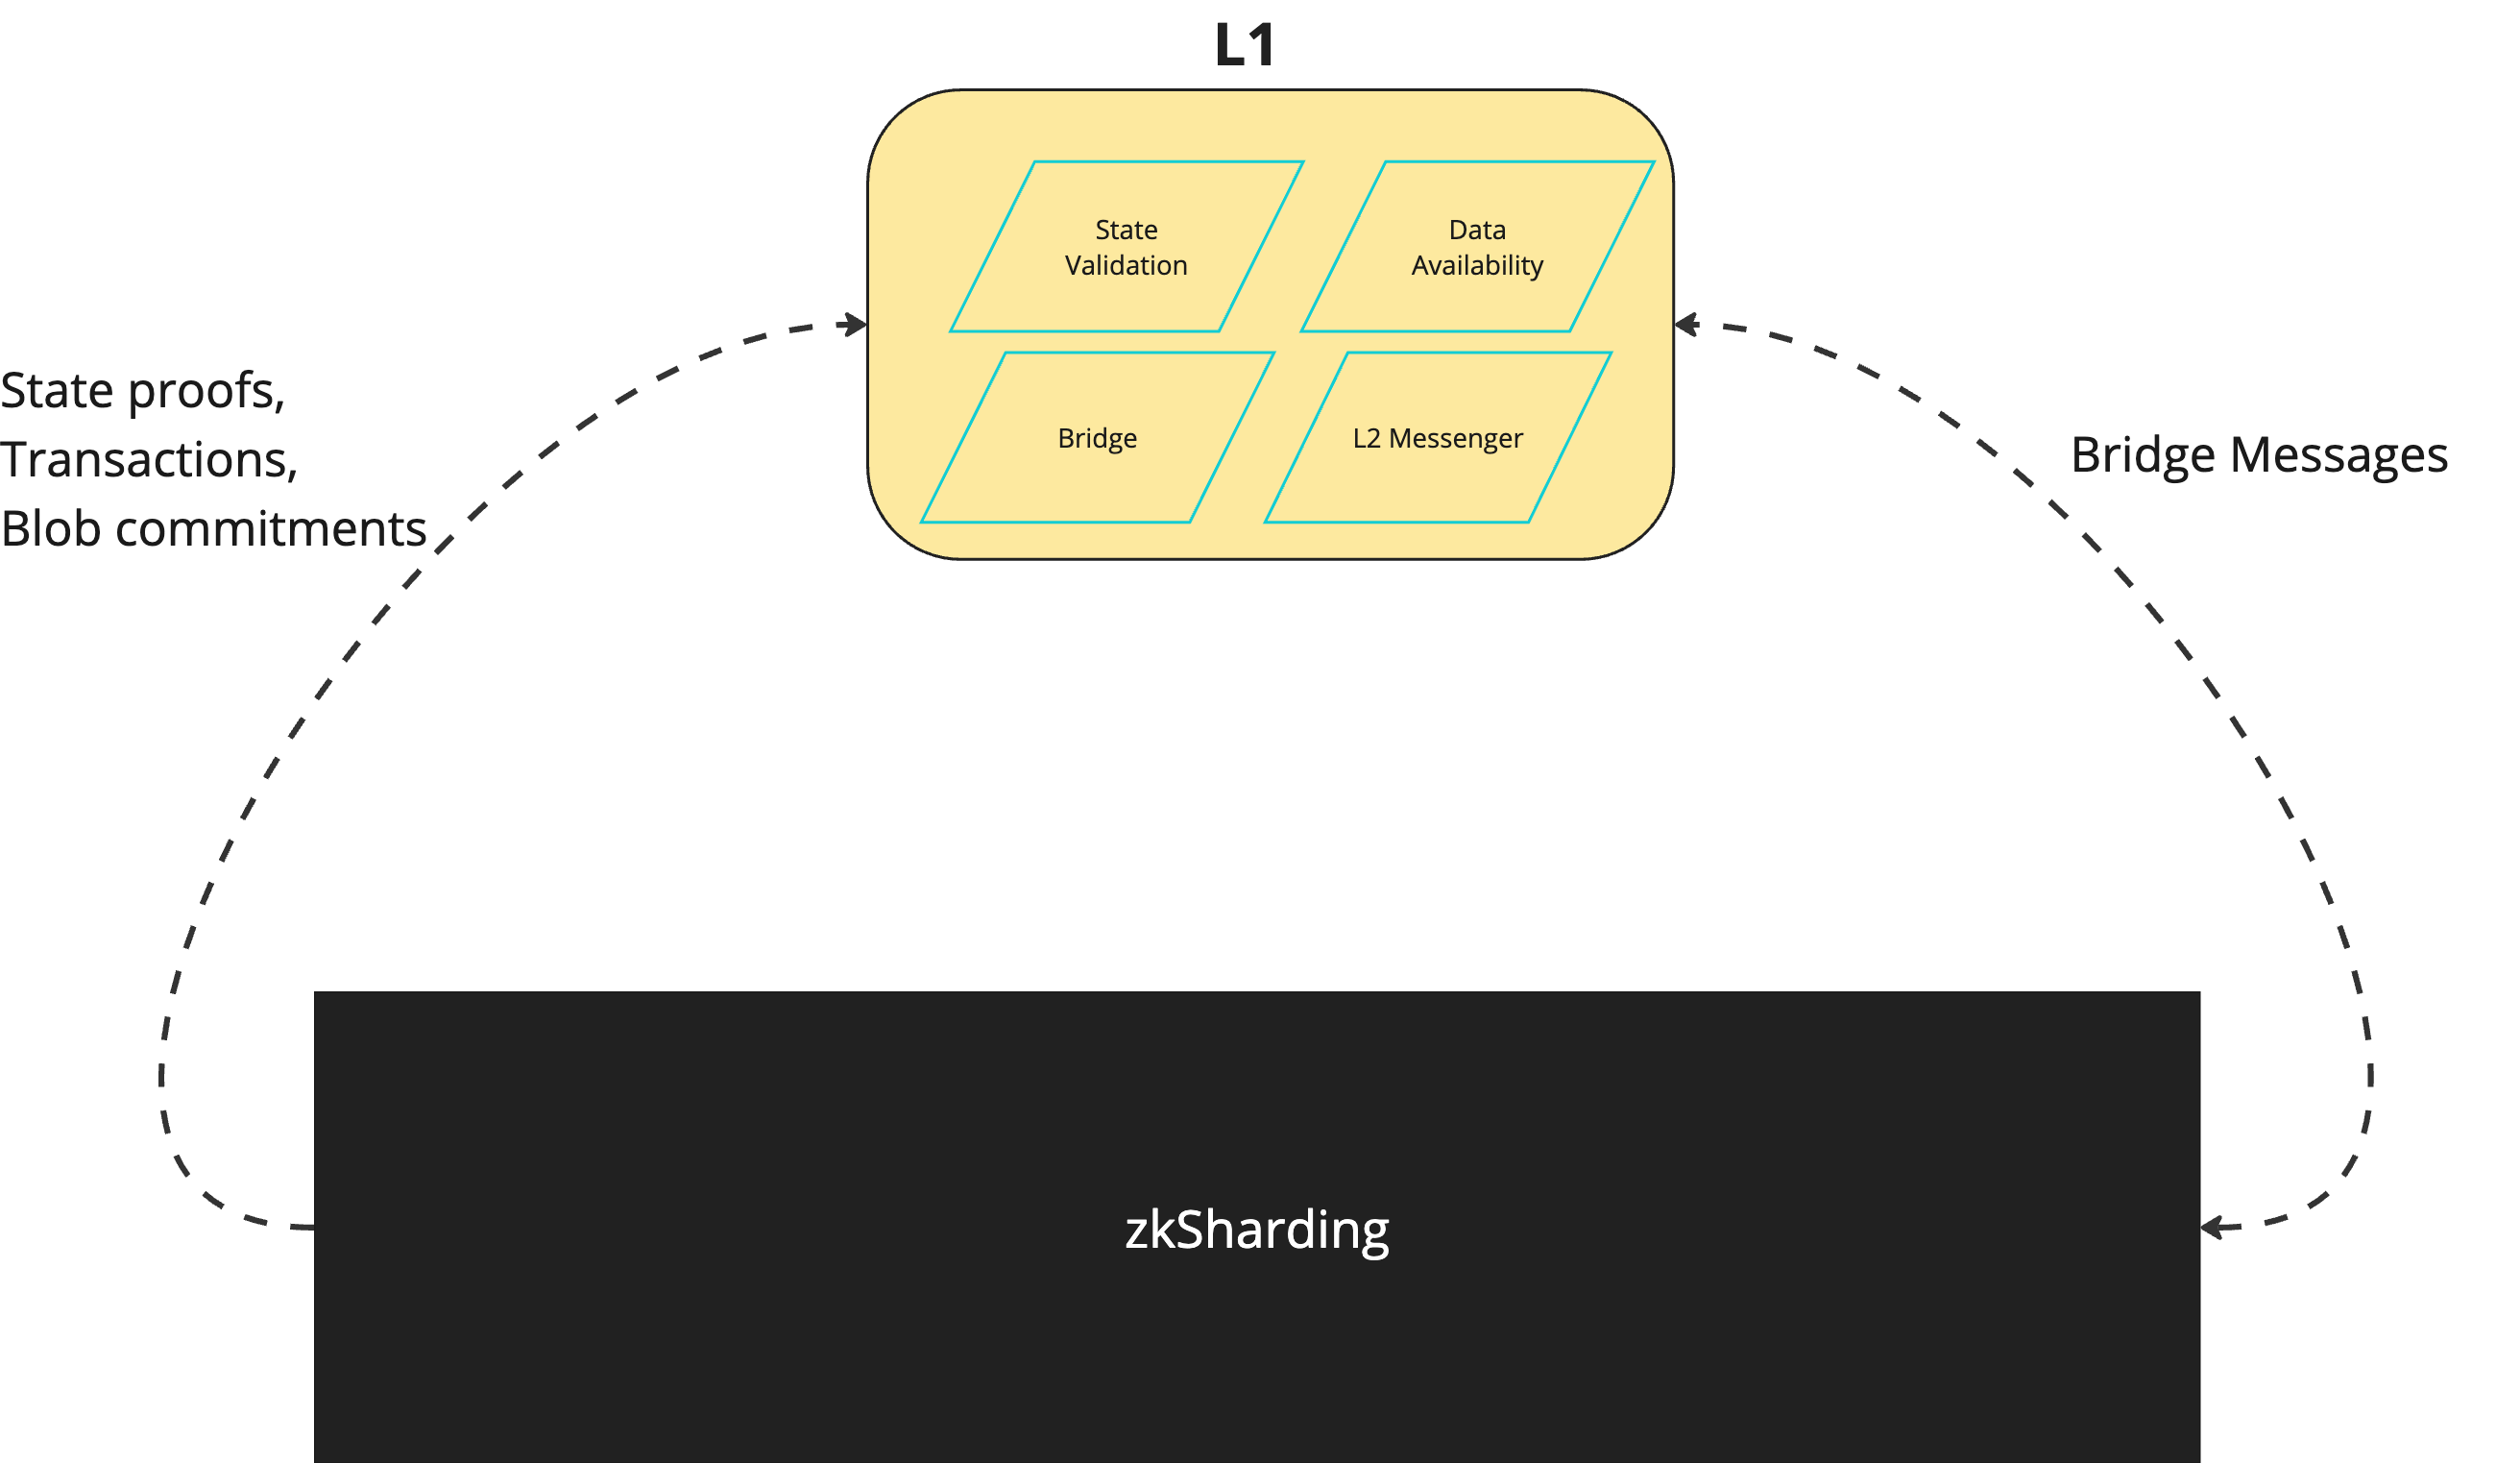
\includegraphics[width=0.5\linewidth]{figures/blackbox}
	\caption{Visualizing zkSharding as a \emph{blackbox}}
	\label{fig:blackbox}
\end{figure}

\short{
	From L1’s perspective (see
	Figure
	\ref{fig:blackbox}), zkSharding is a blackbox which periodically
	submits
	cryptographic proofs and data blobs to verify its operations
	without
	revealing internal processes. L1 provides key contracts for state
	validation, deposits, withdrawals, and data availability. While L1
	provides zkSharding with a reliable settlement layer to verify
	zkSharding's state  and a data availability layer, zkSharding
	enables L1
	to achieve higher throughput by offloading transaction processing
	to
	zkSharding. The L1 network is unaware of the detailed execution
	inside
	zkSharding, but it plays a crucial role in maintaining
	zkSharding’s
	trustworthiness and security.
}{
	Before exploring the design of zkSharding, it is crucial to
	understand
	how zkSharding functions as a rollup on Ethereum’s Layer 1 (L1).
	While
	zkSharding is internally complex, involving multiple shards
	processing
	transactions in parallel, L1 sees zkSharding much like any other
	zkRollup.
	From L1’s perspective, zkSharding periodically submits
	cryptographic
	proofs to verify the correctness of its operations and stores some
	essential data as blobs, without exposing its internal processes.
	Even though L1 is not aware of zkSharding's full internal
	operations or
	shard structure, L1 hosts key contracts that enable zkSharding’s
	integration with Ethereum, including  state validity and handling
	deposits
	and withdrawals. It also provides data availability services to
	the
	zkSharding. While L1 provides zkSharding with a reliable
	settlement layer
	to verify zkSharding's state  and act as a data availability
	layer,
	zkSharding enables L1 to achieve higher throughput by offloading
	transaction processing to zkSharding.
	In essence, one can visualize zkSharding as a \emph{blackbox} (See
	Figure
	\ref{fig:blackbox}) that processes numerous transactions and
	periodically
	submits proofs to L1 for validation. L1 verifies these proofs and
	stores
	essential data, ensuring that zkSharding remains secure and that
	users can
	transfer assets in and out of the system seamlessly. The L1
	network is
	unaware of the detailed execution inside zkSharding, but it plays
	a
	crucial role in maintaining zkSharding’s trustworthiness and
	security.
}

For more insights into zkSharding's internal mechanics and how it achieves
high throughput, refer to the next sections. Now, we introduce the key
functionalities that L1 provides to support zkSharding.

\paragraph{L1 Data Availability:}
\short{
	Proto-Danksharding (EIP-4844) \cite{eip-4844}  is a proposal aimed
	at reducing rollup costs when posting data to Ethereum’s L1.
	zkSharding
	leverages this by utilizing Ethereum's data availability layer.
	zkSharding
	submits executed transactions as a \emph{compressed} batch,
	denoted as
	$\batch^*$, in the form of a data blob. This blob is committed to
	Ethereum’s execution layer via a KZG commitment  \cite{kzg}, which
	represents the data as a polynomial for efficient storage and
	verification. Batch compression is utilized to maximize the number
	of
	transactions that can be efficiently stored within a single blob,
	ensuring
	optimal use of available space.
}{
	Proto-Danksharding (EIP-4844) \cite{eip-4844} is a proposal aimed
	at reducing rollup costs when posting data on Ethereum’s L1.
	zkSharding
	takes advantage of this by utilizing Ethereum's data availability
	layer.
	zkSharding submits the executed transactions, referred to as the
	compressed batch $\batch^*$, in the form of a data blob, which is
	then
	committed to L1’s execution layer using a KZG commitment. A KZG
	commitment
	\cite{kzg} is a cryptographic method that allows Ethereum to
	efficiently
	verify large amounts of data (such as zkSharding’s transaction
	history) by
	representing the blob data as a polynomial. This ensures efficient
	data
	storage while maintaining the ability to verify that zkSharding’s
	transactions are available and valid. zkSharding uses batch
	compression to
	maximize the number of transactions that can be efficiently stored
	within
	a single blob, ensuring optimal use of available space
	\cite{compression}.
}

\paragraph{State Validity Contract:} The State Validity Contract is
crucial for ensuring the correctness of zkSharding's new state after
processing transactions across all shards. It verifies that the new state
correctly reflects the processed transactions, represented by $\batch$,
from \emph{all shards}. When zkSharding submits a new state root $\stroot$
to L1, it also provides a proof $\pi$ to prove the correctness of this new
state. The contract checks this proof against the KZG commitment $\kzg$ to
the compressed batch $\batch^*$ of $\batch$.

More specifically, the State Validity Contract verifies that the new state
root $\stroot$ was created by correctly applying the transactions from the
commitment $\kzg$ to the last verified state $\st'$ with the root
$\stroot'$. Conceptually, the state update process in zkSharding can be
represented by the state transition function $\fstf$, which takes the
current state $\st'$ and a batch $\batch$ of transactions from all shards,
and produces a new state $\st$ with the root $\stroot$ by executing all
the transactions correctly.

The State Validity Contract receives $\stroot$, $\stroot'$, and the proof
$\pi$ as inputs and also accesses the associated polynomial commitment
$\kzg$. It then verifies the following:

\begin{itemize}
	\item there exists $\batch$ such that $\fstf(\st', \batch)$
	      outputs a new state $\st$ with the root $\stroot$, and
	\item $\batch^*$ committed in $\kzg$ is the compressed version of
	      $\batch$.
\end{itemize}

\paragraph{Deposit/Withdrawal Contracts:}
Deposit contract secures asset transfers from Ethereum to
zkSharding.
When users deposit assets like ETH or ERC-20 tokens, they are
locked on L1
and reflected within zkSharding for use on L2.
The Withdrawal Contract handles asset transfers from zkSharding
back to L1. Once zkSharding processes the withdrawal and generates
a
proof, the contract verifies it and releases the assets on
Ethereum,
ensuring a smooth exit to L1.

We have additional operational contracts deployed on L1, but here we focus
on the key ones that ensure the secure functioning of zkSharding.
\short{
}
{
	Currently, we are researching escape hatches for both users and
	validators
	to safeguard against scenarios where zkSharding is compromised by
	a
	supermajority of malicious validators. While the L1 State Validity
	Contract consistently verifies valid transactions, these escape
	hatches
	are crucial for enabling users to withdraw their tokens even if
	the
	zkSharding environment becomes compromised.
}
